\documentclass[11pt,letterpaper]{article}

\usepackage[top=1in,bottom=1in,left=1in,right=1in]{geometry}
\usepackage{algorithm}
\usepackage{algorithmic}
\usepackage{amsmath}
\usepackage{amssymb}
\usepackage{cite}
\usepackage{bm}
\usepackage[usenames]{color}
\usepackage{enumerate}
\usepackage{graphicx}
\usepackage{subfigure}
\usepackage{textcomp}
\usepackage{times}
\usepackage{url}
\usepackage{xr}
\usepackage{xcolor}

\newcommand\todo[1]{\textcolor{red}{#1}}

\newcounter{reviewcounter}
\setcounter{reviewcounter}{1}

\newenvironment{review}
{\noindent {\bf Comment~\arabic{reviewcounter}}:\addtocounter{reviewcounter}{1}\itshape}
{\vspace{0.8em}}

\newenvironment{response}
{\noindent {\bf Response}: \color{black}}
{\color{black} \vspace{1.6em}}

\title{Morris Responses}

\begin{document}

\maketitle

\todo{To-do notes are in red}

%B1)
\begin{review}
The authors do a nice work of calibrating the cameras and measuring noise in the depth camera. However, in page 2 introduction say that this calibration allows for the explicit correspondence between pixels of any modality.  The authors rely on this to annotate data in one modality and propagate labels in the other (at least this is what I understand from later on description of methodology).  However, this is a VERY strong assumption and depends completely on the distance between the cameras, the angles, the distance between object and sensors and the actual object arrangement. From our experience even when imaging co-planar plants (such as young arabidopsis) at a distance of ~70cm even when the camera sensors are really close to each other (less than 5cm) some differences in view are there and occlusions are present.  The authors should comment on this and should show as supportive evidence examples of plants at different growth stages in all 4 modalities in raw and
annotated form to show how close this correspondence is matching and how the propagated labels.  Furthermore, additional supporting evidence could be obtained either by arranging for two external and blind annotators
to label some data (different age, different placement in the tray to show the effect of angle) in another modality (e.g., optical) and then measure inter-observer variability. Then they can propagate annotations from fluorescence to images of that modality and measure agreement. If this agreement is better than the in between rater variability then you could argue that propagating annotations is ok to do and actually beneficial.  Nevertheless, you should definitely mention this limitation of your work. 
\end{review}

\begin{response}
We expanded our description of the labeling and the propagation to other modalities in the paper.  The data labeling is performed in the fluorescence image modality.  The infra-red image is from the same camera and so pixel labeling will be identical.  The labels are propagated to the color and depth modalities using planar homographies.  The homography between the fluorescence image and the color image is calculated by fitting matching features in these modalities, and the homography to the depth image is found by fitting a plane through the 3D plant points.  As the reviewer noted, using these homographies will result in pixel segmentation errors due to parallax for plant regions outside of the modeled planes.  We evaluate these errors qualitatively and quantitatively.  Figure~\ref{fig:LabelAlignment} illustrates the label propagations from the fluorescence image to the other modalities and from the color image to other modalities with two different line colors.  Errors occur where the lines fail to overlap and are due to propagation effects as well as boundary selection variations by the labeler between modalities.  We compare the magnitude of these two effects in table \todo{XXX}. \todo{ADD TABLE RESULTS}


\begin{figure*}
\begin{centering}
\begin{tabular}{cccc}
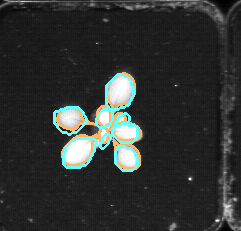
\includegraphics[width=.18\textwidth]{../Figures/LabelAlignment/day_3_hour_23-seg_ir.png}&
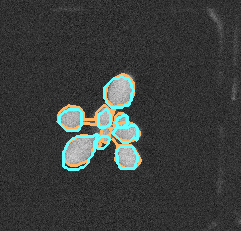
\includegraphics[width=.18\textwidth]{../Figures/LabelAlignment/day_3_hour_23-seg_fmp.png}&
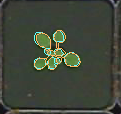
\includegraphics[width=.18\textwidth]{../Figures/LabelAlignment/day_3_hour_23-seg_rgb.png}&
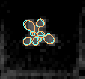
\includegraphics[width=.18\textwidth]{../Figures/LabelAlignment/day_3_hour_23-seg_depth.png}\\
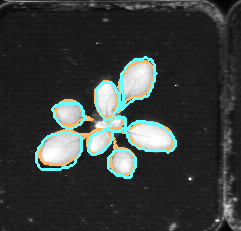
\includegraphics[width=.18\textwidth]{../Figures/LabelAlignment/day_5_hour_23-seg_ir.png}&
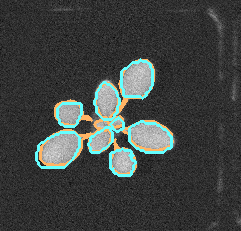
\includegraphics[width=.18\textwidth]{../Figures/LabelAlignment/day_5_hour_23-seg_fmp.png}&
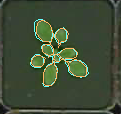
\includegraphics[width=.18\textwidth]{../Figures/LabelAlignment/day_5_hour_23-seg_rgb.png}&
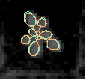
\includegraphics[width=.18\textwidth]{../Figures/LabelAlignment/day_5_hour_23-seg_depth.png}\\
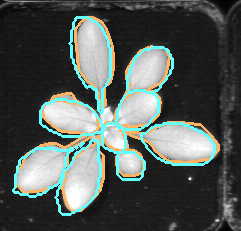
\includegraphics[width=.18\textwidth]{../Figures/LabelAlignment/day_9_hour_20-seg_ir.png}&
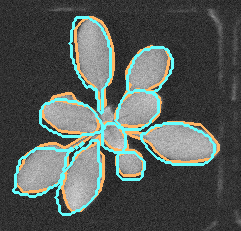
\includegraphics[width=.18\textwidth]{../Figures/LabelAlignment/day_9_hour_20-seg_fmp.png}&
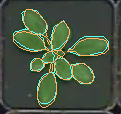
\includegraphics[width=.18\textwidth]{../Figures/LabelAlignment/day_9_hour_20-seg_rgb.png}&
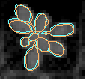
\includegraphics[width=.18\textwidth]{../Figures/LabelAlignment/day_9_hour_20-seg_depth.png}\\
($a$) & ($b$) & ($c$) & ($d$) \\
\end{tabular}
\caption{Label propagation between all four modalities ($a$) infra-red, ($b$) fluorescence, ($c$) color and ($d$) depth, of a sample plant in the Arabidopsis collection for day 3 (top row), day 5 (middle row), and day 9 (bottom row).  In the dataset the manual segmentation is performed on the fluorescence images and is outlined here as orange lines propagated to all modalities.  The infra-red image is taken by the same camera and so will have close to exact pixel correspondence.  To assess the segmented pixel propagation to other modalities, we also manually labeled a subset of the color plant images and propagated this segmentation to all modalities (shown in cyan).  Comparing these boundaries in each modality gives a measure of the propagation errors due to parallax, and we provide quantitative analysis in table XXX.  Note that the color and depth images are rotated 90 degrees.}
\label{fig:LabelAlignment}
\end{centering}
\end{figure*}

\end{response}

%C)
\begin{review}
Fig 3 (a) ... From Fig 2 it appears the distance from plant to sensor to be greater than 60mm (6cm) !!! ie., to me it looks close to 60cm, but either Fig 3 has wrong axis range or something else is going on. Can you please explain/update?
Also same figure (3), shouldn't the images overlap? why are shown translated?  
\end{review}

\begin{response}
Yes, the distance to the plant is roughly 620mm.  The image planes are plotted not at the plant location, but at a distance proportional to the focal length of each camera.  We added dashed lines to the figure to make it clearer that these planes do not correspond to the plant depth, and updated the caption to explain it better.
\end{response}

%E1
\begin{review}
On manual annotation process:  Did you use an extra annotator or a supervisor? 
\end{review}

\begin{response}
We used an extra annotator. \todo{is this correct?}
\end{response}

%E4
\begin{review}
Again going back to the problem of lack of exact 1-1 correspondence between modalities, how can you guarantee that labels on one are good on the other given such high differences in resolutions among modalities?  Please include at least some visual examples.
\end{review}

\begin{response}
The pixel correspondence accuracy evaluation is explained in a response above, and a figure has been added to illustrate it, (Figure~\ref{fig:LabelAlignment}). 
\end{response}

%A
\begin{review}
I do not subscribe to the term dense for such low resolution depth cameras. In my book dense refers to high res depth maps. Maybe the authors can reconsider the use of the term.
\end{review}

\begin{response}
We agree and removed the term dense from the depth map image.
\end{response}


\end{document}


